\documentclass[8pt]{article}

\title {\textbf{Vulkan Renderer}}
\date{June 2022}

\usepackage{amsmath}
\usepackage{blindtext}
\usepackage{caption}
\usepackage{geometry}
\usepackage{graphicx}
\usepackage{hyperref}
\usepackage{multicol}

\geometry{
	a4paper,
	left=20mm,
	%right=
	%bottom=
	top=15mm}


\newenvironment{Figure}
  {\par\medskip\noindent\minipage{\linewidth}}
  {\endminipage\par\medskip}

\begin{document}
		\maketitle

		\begin{figure}[h!]
			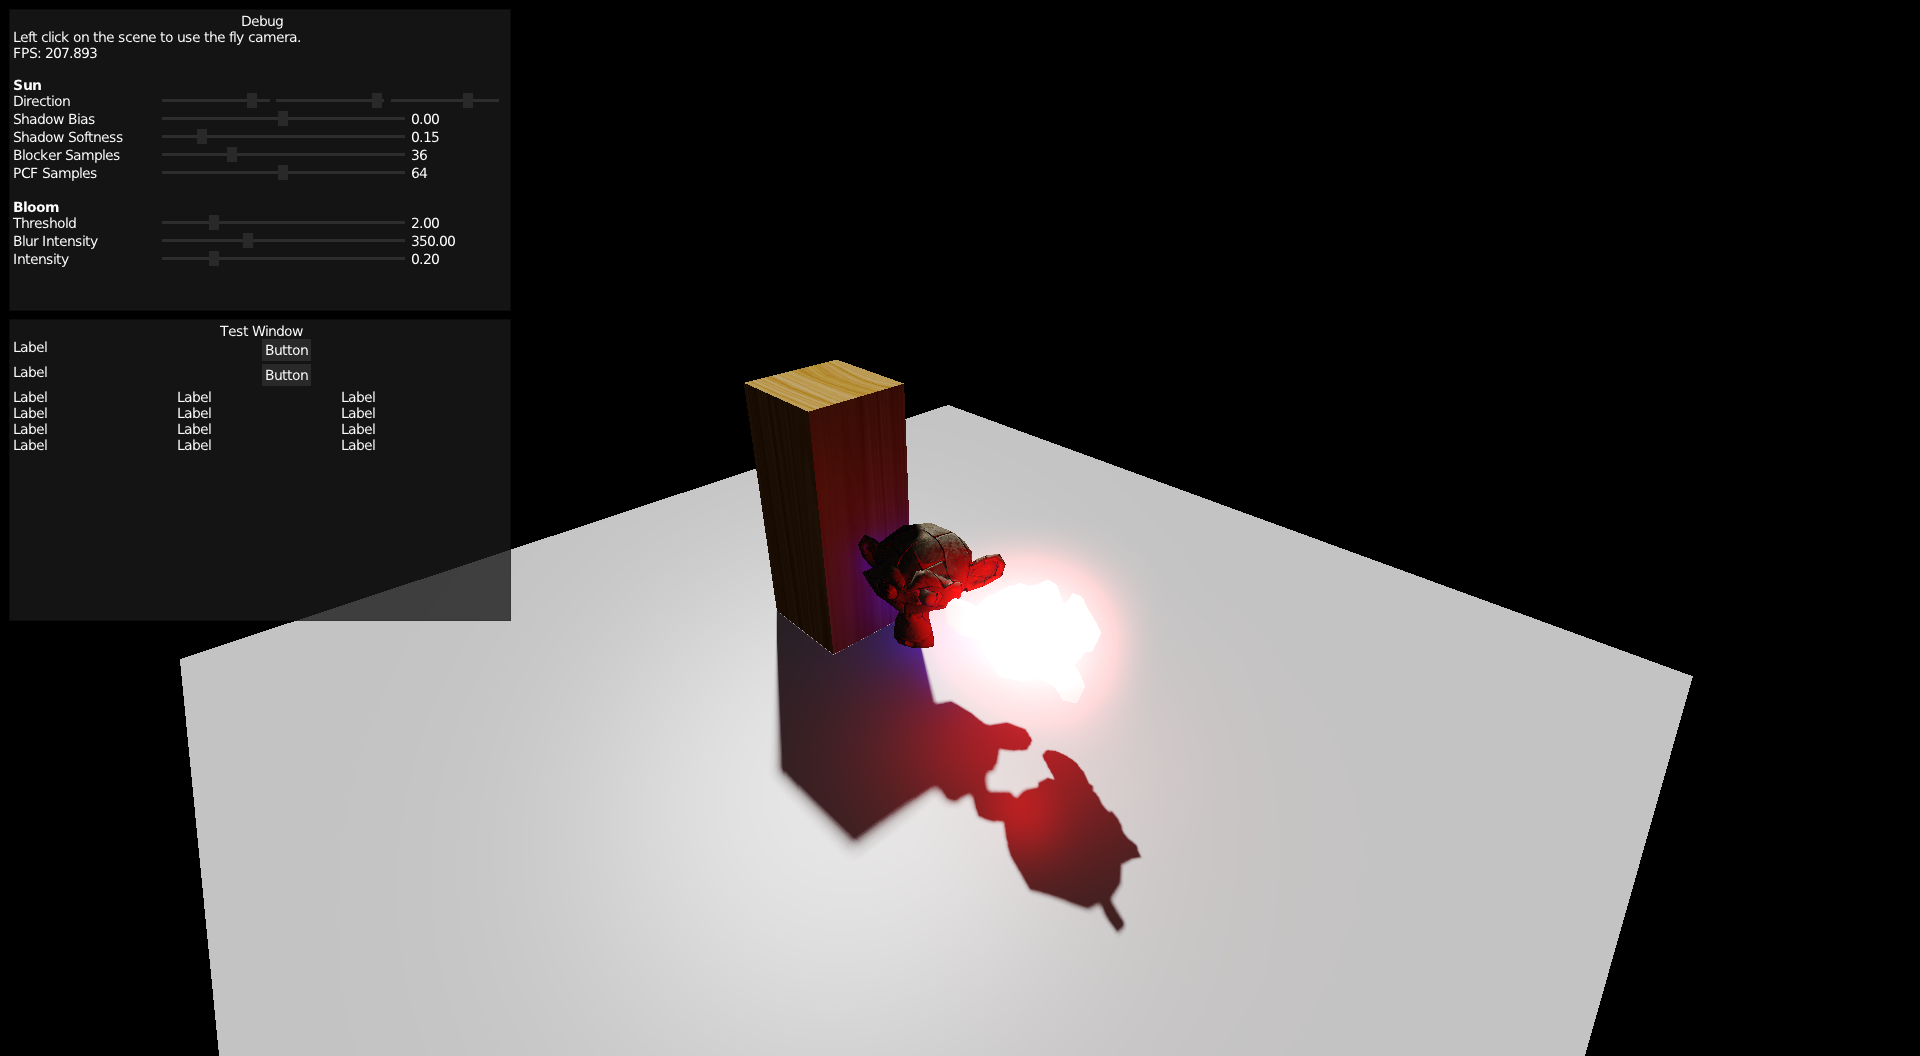
\includegraphics[width=\linewidth]{media/screenshot_001.png}
			\caption{PCSS makes the shadow appear more or less soft depending on the distance of the blocker.}
			\label{fig:pcss}
		\end{figure}

		\begin{multicols}{2}
			\section{Brief}
			The modular system is to be a real-time 3-D renderer that makes use
			of the Vulkan API. It will include the following features: -
			Wavefront loading.  - 3-D lighting including normal mapping and
			soft shadows.  - Simple post-processing effects such as Bloom.

			It will rely on GLFW for windowing and input. The rest is to be
			implemented from scratch in C++.

			The renderer will be built as a dynamic library/shared object, to
			be linked to a client application. This is so that any external
			libraries that the renderer relies on won't have to be linked into
			client applications as well, which would be the case if the
			renderer were linked to clients statically.

			The renderer will make use of various mathematical functions for
			3-D transformation including vector operations such as the dot and
			cross product and matrix operations like translation, rotation,
			scaling and projection matrices. It will also provide soft shadows
			using PCSS and PCF.

			The renderer will provide a base class for applications that
			clients inherit from which provides functionality like abstracting
			the GLFW windowing and input, as well as creating the Vulkan
			instance. The goal is for all Vulkan calls to be abstracted behind
			at least a thin object-oriented layer. For example, a "Mesh" class
			which will manage vertex and index buffers for the user that they
			can simply push data into and draw on command, or a "Scene" class
			that manages different meshes, post processing effects and lights.

			\section{Implementation Overview}
				The final features include:
				\begin{itemize}
					\item Wavefront loader.
					\item 3-D rendering, point lighting and normal mapping using deferred shading.
					\item Percentage-Closer Soft Shadows.
					\item Bloom and tone mapping.
					\item Vulkan API abstraction.
					\item Text rendering and basic GUI.
					\item 2-D rendering using texture atlasing.
				\end{itemize}

			The Vulkan API abstraction creates and object-oriented layer around
			textures and buffers (vertex, index and frame buffers), GLFW
			windows, as well as the graphics pipeline. The Renderer3D and
			Renderer2D classes build abstractions on top of the API abstraction
			to provide extra functionality and provide an easy-to-use layer
			that allows easy rendering of 3-D objects and 2-D sprites.

			The 2-D rendering uses a texture atlasing system that packs all of
			the textures that it requires on the fly, so that the shader only
			ever has to sample a single texture. The algorithm it uses to do
			this is extremely stupid and simply lines up all of the textures
			along the x axis.

			The shadow mapping makes use of a technique named
			"Percentage-Closer Shadow Mapping" (PCSS). This technique samples
			the depth map in terms of the surface to gain an average of how far
			away the shadow blockers are (the "blocker search"). Using that
			average, it uses a formula described in
			\href{https://developer.download.nvidia.com/shaderlibrary/docs/shadow_PCSS.pdf}{this
			paper} to estimate the size of the penumbra of the shadow. Then,
			the shader runs a PCF algorithm on the shadow map with a radius
			that depends on the penumbra size. This has the effect of causing
			the shadow to appear more soft the further away the object blocking
			the light is from the surface that's receiving the shadow. This is
			particularly visible in Figure \ref{fig:pcss}.

			For object management, the renderer relies on the
			\href{https://github.com/quou/ecs}{ECS that I wrote} some time ago.
			This decision was made because I enjoy working with Entity-Component
			architectures and it made for a quick setup.

			\section{Performance Evaluation}
			The 3-D renderer's performance is real-time but not brilliant
			compared to the renderers included in tools such as Unity. This is
			mostly due to the low speed of some of the post processing effects,
			namely Bloom, which samples the texture quite heavily. The
			shadow-mapping uses PCF, which requires a lot of samples to avoid
			unwanted effects such as banding. Another technique that might
			improve speed would be Variance shadow mapping, though that would
			greatly increase the complexity of the system should PCSS also be
			desired, probably requiring the use of a compute shader. With bloom
			and soft-shadows enabled using 36 samples for the shadow blocker
			search and 64 samples for PCF, the renderer can run at between 200
			and 300 FPS on my Radeon RX 570 GPU, running an optimised and stripped
			build from GCC on GNU/Linux.

			The "Sandbox" application provides an example that demonstrates the
			3-D and 2-D renderers and the GUI. It loads a few fonts and 3-D models,
			displays debug and test GUI windows and has a free-moving camera.
			I created this application asynchronously to the library itself. This
			way, I was able to correct errors and bugs in the library quickly.
			
			Some of the bugs, issues and challenges I encountered were:
				\begin{itemize}
					\item Various Vulkan validation errors, some of them taking
						many days to fix, including:
						\begin{itemize}
							\item An error when the window is bigger than the
								screen. This was caused by trying to create a
								frame buffer larger than what the swapchain
								images could provide. It was solved by querying
								the swapchain for the maximum and minimum image
								sizes that it could support.
							\item An error on pipline re-creation caused by
								pushing Vulkan commands to the command buffer
								and then flushing it, even though the pipeline
								corresponding to the commands had been destroyed.
								It was fixed by delaying the pipeline re-creation
								until the beginning of the frame and then
								skipping the rest of that frame. This does cause
								flicking every time the pipeline is re-created,
								but I think that's acceptable since the scenarios
								in which the pipeline is re-created are limited.
						\end{itemize}
					\item Supporting multiple different textures to be bound between
						draw calls took quite a lot of refactoring before I could
						settle on a solution that felt to have acceptable quality,
						which was to create a wrapper around Vulkan descriptors
						that are passed as arrays into the constructor of the
						graphics pipeline abstraction. This means that all materials
						and uniform buffers have to be declared before the pipline
						can be created, however, unlike many OpenGL renderers. I
						think this is fair, though, because in a real-world
						application all of the assets would be loaded first anyhow.
					\item Making the PCF on the shadows look acceptable was
						difficult, as PCF can often cause banding if the sample
						count is not high enough to match the radius, as seen in
						Figure \ref{fig:shadow}. With 64 samples, the shadows look
						good as long as the shadow softness parameter is not too
						high (by default the shadow softness is set to 0.15).
				\end{itemize}

			\begin{Figure}
				\centering
				
\includegraphics[width=\linewidth]{media/shadow.png}
				\captionof{figure}{Zooming into the shadow reveals ugly banding from PCF.}
				\label{fig:shadow}
			\end{Figure}

			Some features that may be interesting but that I didn't get around
			to are:
				\begin{itemize}
					\item Shader hot-reloading. Currently, I have a small Lua
						script that I wrote that parses shader files, performing
						some pre-processing and then and invoking a call to
						\texttt{glslc} to compile them into SPIR-V bytecode.
						It would be nice to use the SPIR-V C++ library to
						pre-process and compile the shaders from within the
						application. This would also allow shaders to be
						hot-reloaded more cleanly, as well.
				\end{itemize}
		\end{multicols}
\end{document}
